\begin{tikzpicture}[
			window/.style={draw=red, dashed, line width=0.6pt},
			condtag/.style={draw=none, fill=none, inner sep=1.7pt,
					font=\scriptsize, text=black, align=center,
					text height=1.5ex, text depth=0.25ex}
		]
		\node[inner sep=0] (wave) {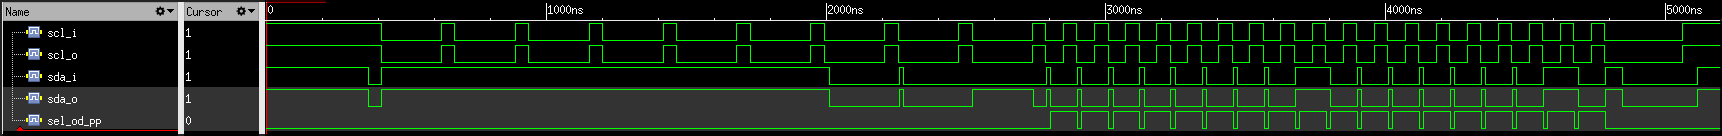
\includegraphics[width=\textwidth]{enec/enec_bcast.png}};
		\begin{scope}[shift={(wave.south west)},
				x={($(wave.south east)-(wave.south west)$)},
				y={($(wave.north west)-(wave.south west)$)}]
			\draw[window] (0.198,-0.14) rectangle (0.238,1.14);
			\draw[window] (0.243,-0.14) rectangle (0.6095,1.14);
			\draw[window] (0.6145,-0.14) rectangle (0.7719,1.14);
			\draw[window] (0.7769,-0.14) rectangle (0.948,1.14);
			\draw[window] (0.953,-0.14) rectangle (1.000,1.14);
			\node[condtag, anchor=south] at (0.218,1.16) {S};
			\node[condtag, anchor=south] at (0.42625,1.16) {Broadcast Address};
			\node[condtag, anchor=north] at (0.42625,-0.16) {0x7E, RnW = Write};
			\node[condtag, anchor=south] at (0.6932,1.16) {CCC};
			\node[condtag, anchor=north] at (0.6932,-0.16) {0x00};
			\node[condtag, anchor=south] at (0.86245,1.16) {Event Byte};
			\node[condtag, anchor=north] at (0.86245,-0.16) {0x01};
			\node[condtag, anchor=south] at (0.9765,1.16) {P};
		\end{scope}
	\end{tikzpicture}
